\section{Memory Organization}
\label{sec:memory}

The central context of SGX is the \textit{enclave}, a protected environment
that contains the code and data pertaining to a security-sensitive computation.
This section provides an overview of the data structures used by an enclave.


\subsection{Memory Ownership vs Management}

% Access Control Requirements: SGX S 2.3

Enclaves use RAM to store their code and data, and need logical processors to
execute their code in order to perform the computation they were designed to
do. These computer resources are traditionally managed by privileged software,
such as hypervisors and operating system kernels.

In order for SGX to fit into this design, the code inside SGX enclaves is
subjected to the same address translation mechanism (\S~\ref{sec:paging}) as
the applications that enclose the enclaves. Enclave code runs at ring 3
(\S~\ref{sec:rings}), just like application code, so that it cannot
interfere with the privileged software that manages resources.

% Interactions with VMX: SGX S 6.5, 6.5.{1,2,3,4,5}

The rest of the paper will use the term \textit{system software} to refer to
the privileged software that manages resources. On most computers, this is an
operating system kernel. When VMX is in use, SGX resources are allocated by
the hypervisor to guest operating systems running in virtual machines.


\subsection{Enclaves in RAM}
\label{sec:prm}

% PRM: SGX S 3.5
% Interactions with DMA: SGX S 6.10
% Interactions with Memory Configuration: SGX S 6.11

The enclaves' code and data is stored in \textit{Processor Reserved Memory}
(PRM), a contiguous range of RAM that cannot be directly accessed by other
software, including privileged software such as the SMM code, the hypervisor,
and the OS kernel. The memory controller is integrated on the CPU die (see
Figure~\ref{fig:cpu_die}), so it can be trusted to prevent devices attached to
the system bus from performing DMA transfers to/from the PRM.

\begin{figure}[hbt]
  \center{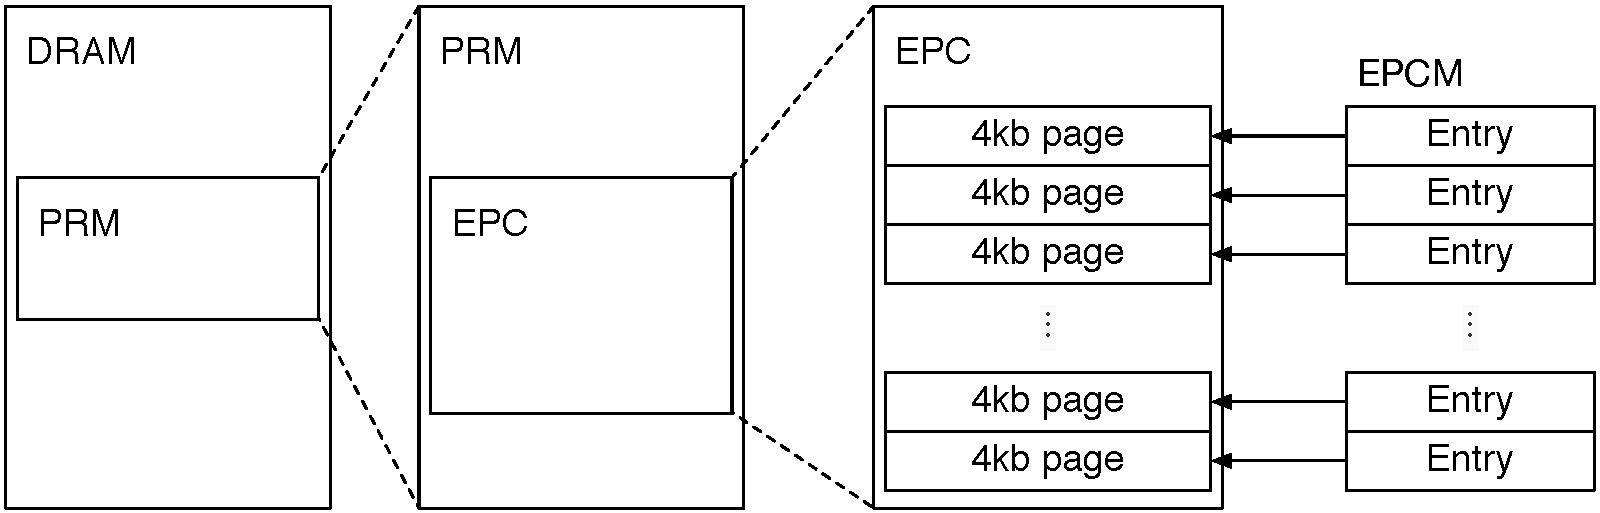
\includegraphics[width=85mm]{figures/sgx_epc.pdf}}
  \caption{
    Enclave data is stored into the EPC, which is a subset of the PRM. The
    PRM is a contiguous range of RAM that cannot be accessed by system software
    or peripherals.
  }
  \label{fig:sgx_epc}
\end{figure}

Rejecting improper accesses to PRM is central to the SGX security model. The
designers were aware of that, and took clear steps to reduce the complexity of
the PRM checks, which in turn reduces the probability of bugs in the
implementation. The PRM must be set up to use SGX features and, once
configured, the PRM range cannot be changed. Furthermore, the PRM's size must
be an integer power of two, and its start address must be aligned to the same
power of two. The range restrictions reduce the complexity of checking if a RAM
address is in the PRM to a bitwise AND and an equality comparison.


\subsection{The Enclave Page Cache (EPC)}
\label{sec:epc}

% EPC and EPCM: SGX S 1.5, S 1.5.1, S 2.6.13, S 3.5, S 3.5.1

The contents of enclaves and the associated data structures are stored in the
\textit{Enclave Page Cache} (EPC), which is a subset of the PRM.

The SGX design handles multiple enclaves active at the same time, which is
necesssary in multi-tasking environments. This is achieved by having the EPC
split into 4kb pages, which can be associated to different enclaves. The system
software uses SGX instructions to allocate unused pages to enclaves, and to
free previously allocated EPC pages. SGX also offers a method for system
software to evict EPC pages into non-EPC memory, which allows the EPC to be
over-committed, just like evicting pages to disk (swapping) allows the main
memory to be over-committed.

Normally, system software manages physical memory by directly modifying the
contents of page tables, and is responsible for ensuring that the state not
covered by cache coherency is synchronized across logical processors, by
performing TLB shootdowns (\S~\ref{sec:tlbs}, \S~\ref{sec:cache_coherence}). If
the system software does not perform a TLB shootdown correctly, application
software can experience race conditions. In the context of SGX, one such race
condition is having an EPC page simultaneously accessible by two different
enclaves, which would compromise the SGX security guarantees. Therefore, the
SGX instructions used for EPC management ensure that TLBs are invalidated
properly.

The SGX instructions that allocate a page to an enclave also copy data from a
page outside PRM to the EPC page. Non-enclave software is not permitted to
access the PRM, so the page allocation instructions provide the only
opportunity for system software to load the initial code and data into an
enclave.

\subsubsection{The Enclave Page Cache Map (EPCM)}
\label{sec:epcm}

The CPU maintains some metadata for each EPC page into the \textit{Enclave Page
Cache Map} (EPCM). The metadata tracks the enclave that each page was allocated
to, so the processor can prevent the code inside an enclave from accessing EPC
pages that belong to other enclaves. Table~\ref{fig:epcm_entry} shows the
contents of an EPCM entry.

% EPCM table: SGX S 2.6.13

\begin{table}[hbt]
  \center{\begin{tabularx}{\columnwidth}{| l | r | X |}
  \hline
  \textbf{Field} & \textbf{Bits} & \textbf{Description}\\
  \hline
  VALID & 1 & 0 for un-allocated EPC pages \\
  \hline
  BLOCKED & 1 & page is being evicted (\S~\ref{TBD})\\
  \hline
  R & 1 & allow reads by enclave code\\
  \hline
  W & 1 & allow writes by enclave code\\
  \hline
  X & 1 & allow execution of code inside the page, inside enclave\\
  \hline
  PT & 8 & page type (\S~\ref{sec:key_structures})\\
  \hline
  ADDRESS & 48 & the linear address used to access this page\\
  \hline
  EID & 64 & identifies the enclave owning the page\\
  \hline
  \end{tabularx}}
  \caption{
    The fields in an EPCM entry.
  }
  \label{fig:epcm_entry}
\end{table}


% Access Control Requirements: SGX S 2.3

The EPCM metadata for a page includes the expected linear address used to
access the page (ENCLAVEADDRESS in Intel's documentation). This address must be
specified when a page is allocated, and cannot be changed until the page is
freed.

When the result of a memory address translation is a physical address of an EPC
page, the CPU ensures\footnote{A mismatch triggers a General Protection Fault.}
that the linear address used in the address translation matches the expected
linear address recorded in the page's EPCM entry. This prevents the system
software, which manages the page tables and EPT, from mapping pages to
unexpected addresses inside an enclave's address space.

A page's EPCM entry also records a \textit{type} (PT) for each page.
Table~\ref{fig:pt_values} shows currently defined types. The EPC pages that
store an enclave's code or data have their type set to \textit{regular}
(PT\_REG in the Intel documentation). Each page that is dedicated to an SGX key
data structure has its EPCM entry's type set to the kind of data structure
stored in the page.  An EPC page's type is set when the page is allocated, and
is immutable throughout the page's lifetime.

\begin{table}[hbt]
  \center{\begin{tabularx}{\columnwidth}{| l | l | X |}
  \hline
  \textbf{Type} & \textbf{Created by} & \textbf{Description}\\
  \hline
  PT\_REG & EADD & enclave code / data \\
  \hline
  PT\_SECS & ECREATE & SECS (\S~\ref{sec:secs}) \\
  \hline
  PT\_TCS & EADD & TCS (\S~\ref{sec:tcs}) \\
  \hline
  PT\_VA & EPT & VA (\S~\ref{sec:va}) \\
  \hline
  \end{tabularx}}
  \caption{Values of the PT (page type) field in an EPCM entry.}
  \label{fig:pt_values}
\end{table}


The SGX documentation does not state where the EPCM is stored, but we can
hypothesize that it is either an on-chip memory, like the L3 cache, or stored
in a PRM region that is not used by the EPC. The exact layout of an EPCM entry
is not defined either, but Table~\ref{fig:epcm_entry} suggests that each entry
takes up 16 bytes, with most fields packed in the bottom 12 bits and top few
bits of the expected linear address.

% SECINFO: SGX S 2.6.5, S 2.6.5.{1,2}


\subsection{Key SGX Structures}
\label{sec:key_structures}

% Access Control Requirements: SGX S 2.3

Pages that store key SGX structures cannot be accessed directly, even by the
code executing inside their enclaves. Furthermore, the SGX instructions that
operate on SGX data structures check the EPCM type fields of their inputs
against the expected types. This type system prevents software from
intentionally or accidentally corrupting the key SGX data structures.

The type-based access restrictions have the desirable side-effect of hiding the
contents of the EPC pages holding key SGX structures from software, so the
internal layout of any key data structure can change across new CPU revisions.
Software cannot access the key structures in EPC, so it cannot become dependent
on a specific processor's implementation details.

The SGX documentation does specify a software-visible layout for each key data
structure. This layout is used by the non-EPC page used to initialize the key
data structure when it is created. Therefore, new CPU revisions must preserve
the ability to initialize the key data structures from the less flexible
software-visible layout.

\begin{figure}[hbt!]
  \center{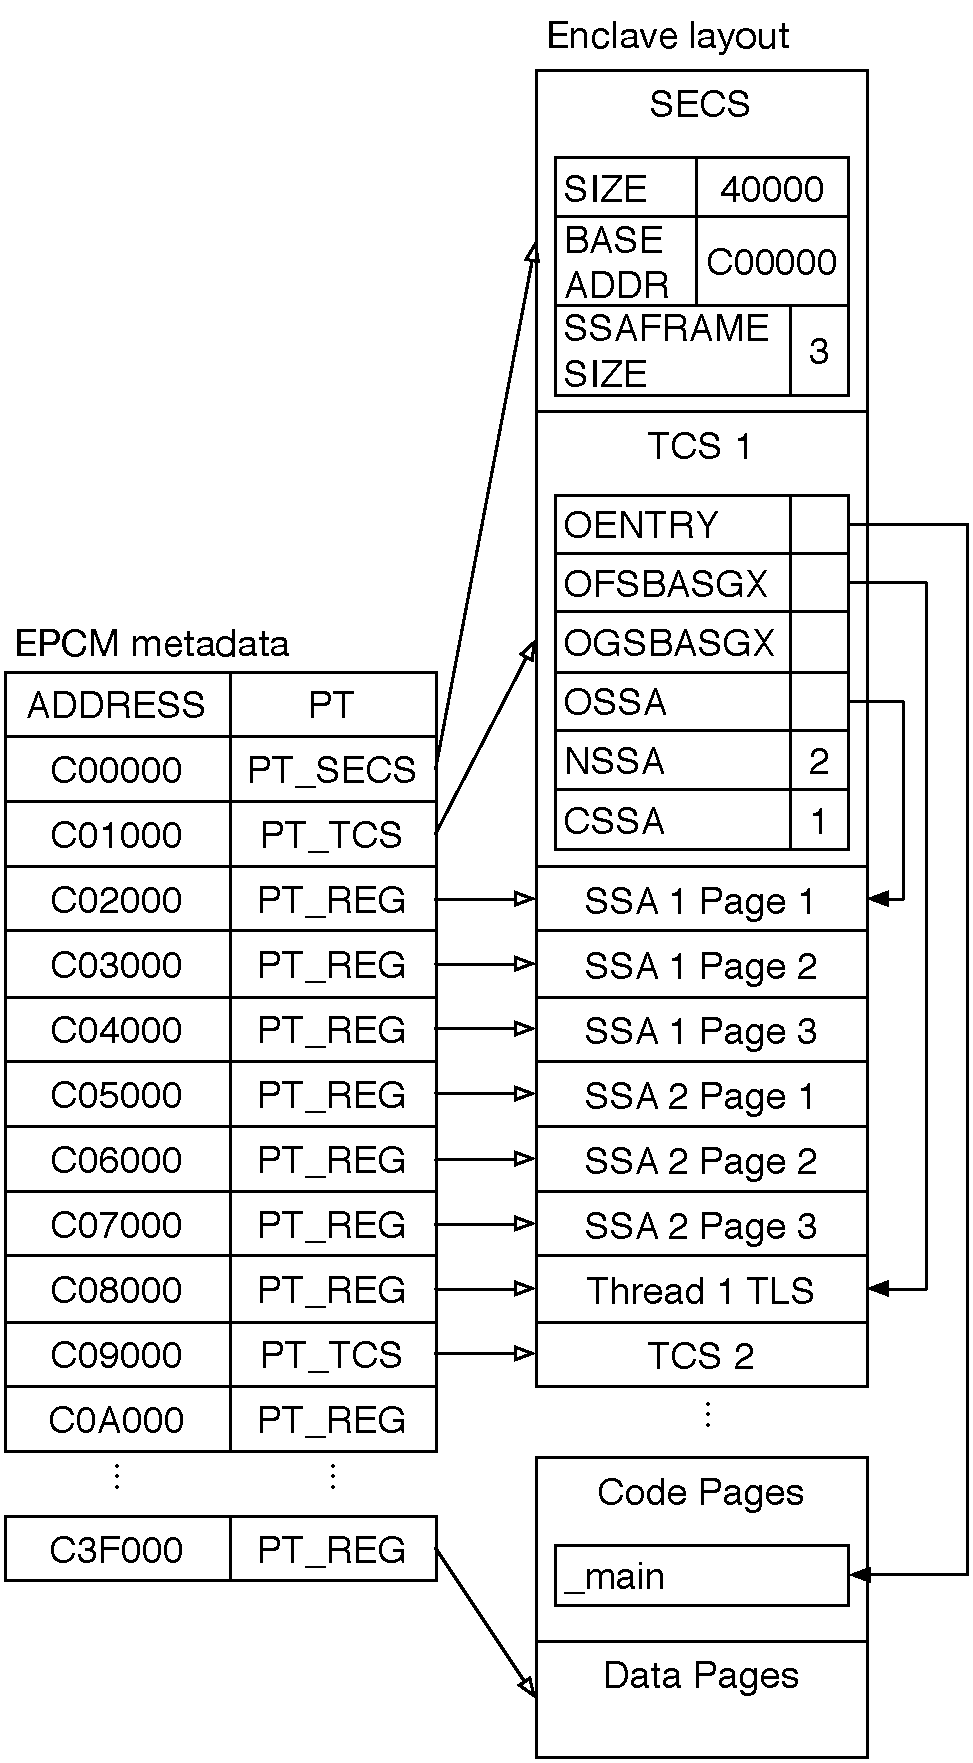
\includegraphics[width=85mm]{figures/enclave_layout.pdf}}
  \caption{
    An enclave's memory layout. Each enclave has a SECS, and one TCS per
    supported hardware thread. Each TCS points to a sequence of SSAs, and
    specifies initial values for RIP, FS and GS.
  }
  \label{fig:sgx_epc}
\end{figure}

\subsubsection{The SGX Enclave Control Structure (SECS)}
\label{sec:secs}

% Main data structures: SGX S 1.4
% SECS: SGX S 2.6.1, S 2.6.1.1, S 3.1
% ECREATE: SGX S 3.1, S 5.3
% Implicit access: SGX S 2.3

The first step in creating an enclave is using the \texttt{ECREATE} instruction
to designate a previously unused EPC page as the enclave's \textit{SGX Enclave
Control Structure} (SECS). All instructions that operate on an enclave access
its control structure directly or indirectly.

The most important field in the SECS is the 64-bit enclave ID (EID), which is
generated by \texttt{ECREATE}. The EID identifies an enclave's pages in the
EPCM, so it must be unique across all active enclaves. EID is documented, but
not included in the software-visible SECS layout.

The software-visible SECS layout has two fields (BASEADDR and SIZE) that
specify the enclave's linear address space (ELRANGE in the Intel
documentation). The enclave's starting address has to be aligned by the enclave
size, which simplifies checking if a linear address belongs to an enclave or
not, just like in the case of PRM physical addresses.

% SECS.ATTRIBUTES.XFRM: SGX S 6.7.2.1

The software-visible SECS also has an ATTRIBUTE field that specifies the Intel
achitecture features used by the enclave code. For example, the MODE64BIT flag
is set if the enclave uses 64-bit code, and the XFRM sub-field contains the
XCR0 register value expected by the enclave's code. XCR0 controls Intel
architecture extensions such as SSE and AVX (see \S~\ref{sec:registers}). When
a logical processor executes code inside an enclave, it uses the XCR0 value
specified by the enclave's SECS, so malicious system software cannot enable
features that the enclave code is not prepared to handle. This frees Intel to
introduce extensions that change the behavior of existing instructions, such as
Memory Protection Extensions (MPX).

The other fields in the software-visible SECS layout are used by the
attestation process, which is explained in \S~\ref{sec:attestation}.

\subsubsection{The Thread Control Structure (TCS)}
\label{sec:tcs}

% TCS: SGX S 2.6.2, S 2.6.2.{1,2,3,4}

A logical processor uses a \textit{Thread Control Structure} (TCS) while
executing code inside an enclave, so enclaves must have at least as many TCS
instances as the number of simultaneous hardware threads that they want to
support.

The fields in the software-visible TCS layout direct the context switches
performed by a logical processor when it transitions between non-enclave and
enclave code.

% SSA: SGX S 2.6.3

In some cases (e.g., when receiving an interrupt), the processor needs to
preempt the execution of enclave code and start running kernel code. This is
accomplished by saving the enclave's context (register values) to an area
inside the enclave, called a \textit{State Save Area} (SSA).

Each TCS references a contiguous sequence of SSAs -- the OSSA field points to
the first SSA, and the NSSA field indicates the sequence's length. When a
logical processor needs to preempt enclave code, it uses the next available
SSA, indicated by the CSSA field in the TCS. The CPU refuses to execute enclave
code using a TCS where no SSA is available (CSSA $\ge$ NSSA).

An SSA essentially consists of the values of the general-purpose registers
(GPRs), and the result of running XSAVE (\S~\ref{sec:registers}) using the
feature mask specified in the ATTRIBUTES.XFRM field in the enclave's SECS.

% SECS.SSAFRAMESIZE: SGX S 6.7.2.2

Each SSA starts at the beginning of an EPC page, and takes up a fixed number of
EPC pages, specified in the SSAFRAMESIZE field in the enclave's SECS. The SSA
alignment and size restrictions most likely exist to simplify the SGX
implementation.

The TCS is stored in a page whose EPCM entry has the type PT\_TCS, and
therefore cannot be directly accessed by enclave software. However, SSAs are
stored in regular pages, so they are accessible to enclave software, and their
layout is defined in the SGX documentation.

\subsubsection{The Version Array (VA)}
\label{sec:va}

Kernels can use the address translation feature (\S~\ref{sec:paging}) in the
Intel architecture to implement virtual memory, where rarely used pages of RAM
are evicted to cheaper but slower memory (usually a hard disk) while they are
not accessed. Virtual memory allows software developers to write applications
as if the computer's main memory is virtually unlimited.

Similarly, SGX includes support for system software to evict EPC pages to
non-EPC RAM, making it possible to have enclaves whose memory requirements
exceed the computer's EPC size.



% VA: SGX S 2.6.12
% EPC and Management of EPC Pages: SGX S 3.5, 3.5.{2,3,4,5,6}



% EPA: SGX S 5.3 EPA

